\documentclass{article}
\usepackage{amsmath}
\usepackage{amssymb}
\usepackage{graphicx}
\usepackage{hyperref}
\usepackage[version=4]{mhchem}

\title{Example 1}
\date{}

\begin{document}
\maketitle

\(A B C\) is an isosceles triangle with \(A B=A C\). Circle \(O\) is drawn using \(A B\) as the diameter to intersect \(B C\) at \(D\). Show that \(B D=D C\).

Solution:
Connect \(A D\).\\
Since \(A B\) is the diameter, \(\angle B D A=90^{\circ}\). So\\
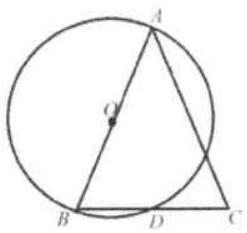
\includegraphics[width=\textwidth]{images/problem_image_1.jpg} \(A D \perp B C\).\\
Since \(A B=A C, A D\) is the perpendicular bisector of \(B C\).\\
Thus, \(B D=D C\).\\
\centering
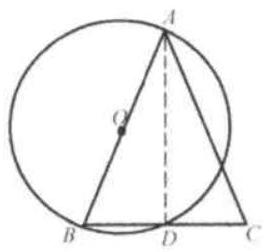
\includegraphics[width=\textwidth]{images/reasoning_image_1.jpg}


\end{document}
